\documentclass{article}

\renewcommand{\labelenumii}{\theenumii}
\renewcommand{\theenumii}{\theenumi.\arabic{enumii}.}

\usepackage{graphicx}
\graphicspath{{Figures/}}

\title{Software Requirements Specification}
\date{24 February 2017}
\author{Team Dodger}

\begin{document}
	\pagenumbering{gobble}
	\maketitle
	\newpage
	\tableofcontents
	\newpage
	\pagenumbering{arabic}
	
	\section{Introduction}
	\subsection{Purpose}
	\subsection{Scope}
	\subsection{Definitions, Acronyms and Abbreviations}
	\subsection{References}
	\subsection{Overview}
	
	\section{Overall Description}
	\subsection{Product Perspective}
	\subsection{Product Function}
	\subsection{User Characteristics}
	\subsection{Constraints}
	\subsection{Assumptions and Dependencies}
	
	\section{Specific Requirements}
	This section expands on the functional requirements of the system. It gives a detailed 	description of the system and all of its use cases.
	
	\subsection{External Interface Requirements}
	
	\subsection{Functional Requirements}
	This section includes all functional requirements in detail. It includes all use case diagrams, Actor-System interaction diagrams as well as a traceability matrix.	
	
	\subsubsection{Use cases}
	\begin{enumerate}
		\item \underline{Navigation Subsystem}
			
		
	\begin{enumerate}
		\item Get current location
		\begin{enumerate}
			\item \textbf{Description:} The NavUP system must be able to determine a user’s location at any point in time while the user is on the Hatfield campus. The location must be determined regardless of whether the user is indoors or outdoors.
			\item \textbf{Precondition:} The user must have an active account and must be within range of WiFi routers.
			\item \textbf{Postcondition:} The user’s location is determined and displayed.\newline
		\end{enumerate}
		
		\item Search location
		\begin{enumerate}
			\item \textbf{Description:} The NavUP system must provide functionality that enables a user to search for any location (lecture hall, day-house, restaurant) on the Hatfield Campus.
			\item \textbf{Precondition:} The user must have an active account
			\item \textbf{Postcondition:} Matching locations are returned to the user. If no buildings match the search criteria, an appropriate error message is displayed.\newline
		\end{enumerate}
		
		
		\item View location details
		\begin{enumerate}
			\item \textbf{Description:} The NavUP system must allow users to view details related to specific locations. This could include restaurant menus, lecture hall timetable schedules as well as images of the buildings.
			\item \textbf{Precondition:} The user must have an active account and a valid location must be selected on the map.
			\item \textbf{Postcondition:} Relevant location details shown to user.\newline
		\end{enumerate}
		
		\item View places of interest
		\begin{enumerate}
			\item \textbf{Description:} The NavUP system must be able to display places of interests to a user based on their current location. This will include places like restaurants and day-houses that must be displayed in a list form. 
			\item \textbf{Precondition:} The user must have an active account and their current location must be known.  
			\item \textbf{Postcondition:} Relevant places of interest are listed and displayed to the user based on their location.\newline
		\end{enumerate}
		
		\item Navigate to location
		\begin{enumerate}
			\item \textbf{Description:} The NavUP system must be able to provide directions and navigate to a location given the user’s current location as well as a desired destination. The system should calculate the most optimal route by looking at the shortest path as well as pedestrian traffic.
			\item \textbf{Precondition:} The user must have an active account. The user’s current location must be known and the must have specified a destination through the search interface.
			\item \textbf{Postcondition:} The user is provided with directions from their current location to their desired destination.\newline
		\end{enumerate}
		
		\item Show pedestrian traffic
		\begin{enumerate}
			\item \textbf{Description:} The NavUP system must be able to display pedestrian traffic on campus in the form of a heatmap. When navigating to a specified location, the system must show traffic on that specific route. A user should also be able to view an overall heatmap of the campus to see traffic.
			\item \textbf{Precondition:} Users must all have the NavUP app installed and must be registered in order for them to show up on the heatmap.
			\item \textbf{Postcondition:} A heatmap of the campus is displayed. 
		\end{enumerate}
	\end{enumerate}
		\begin{figure}[h!]
		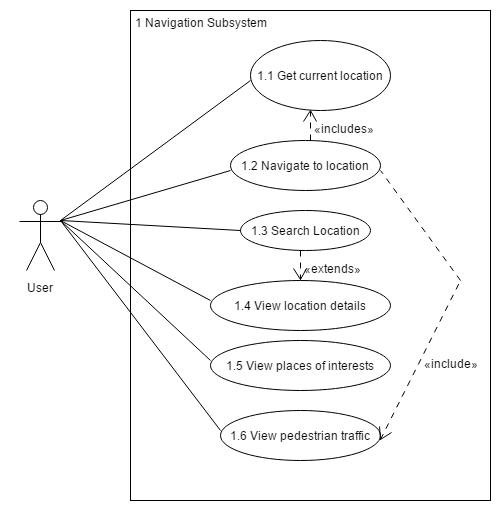
\includegraphics[scale=0.5]{Navigation_Subsystem.png}
		\caption{Navigation Subsystem}	
	\end{figure}
	\item \underline{Location Management Subsystem}
	\item \underline{User Account Management Subsystem}
	
	\item \underline{Entertainment Subsystem}

	
	\item \underline{Achievements Subsystem}
	\item \underline{Administration Subsystem}
	\end{enumerate}
	
	
	\subsection{Performance Requirements}
	\subsection{Design Constraints}
	\subsection{Software System Attributes}
	\subsection{Other Requirements}

\end{document}